\documentclass[11pt]{article}
\usepackage[margin=1in]{geometry}
\usepackage[T1]{fontenc}
\usepackage{lmodern}
\usepackage{microtype}
\usepackage{amsmath,amssymb,amsthm}
\usepackage{graphicx}
\usepackage{booktabs}
\usepackage{tabularx}
\usepackage{multirow}
\usepackage{array}
\usepackage{longtable}
\usepackage{enumitem}
\usepackage[table]{xcolor}
\usepackage[numbers,sort&compress]{natbib}
\usepackage[colorlinks=true,linkcolor=blue!50!black,citecolor=blue!50!black,urlcolor=blue!50!black]{hyperref}
\usepackage{caption}
\captionsetup{font=small,labelfont=bf}
\setlist{itemsep=2pt,topsep=3pt}
\emergencystretch=3em
\usepackage{xurl}

\newtheorem{definition}{Definition}
\newtheorem{proposition}{Proposition}
\newtheorem{corollary}{Corollary}
\theoremstyle{remark}
\newtheorem*{remark}{Remark}

% ---- evidence tags ----
\definecolor{tD}{HTML}{1b7f5a}\definecolor{tS}{HTML}{2a78d6}\definecolor{tN}{HTML}{c0392b}
\definecolor{tH}{HTML}{7a5ab8}\definecolor{tP}{HTML}{8a6d00}\definecolor{tR}{HTML}{52514e}
\newcommand{\etag}[2]{\textsf{\scriptsize\textcolor{white}{\colorbox{#1}{\strut #2}}}}
\newcommand{\Dem}{\etag{tD}{DEMONSTRATED}}
\newcommand{\Sug}{\etag{tS}{SUGGESTIVE}}
\newcommand{\Neg}{\etag{tN}{NEGATIVE}}
\newcommand{\Hyp}{\etag{tH}{HYPOTHESIS}}
\newcommand{\Pro}{\etag{tP}{PROPOSED}}
\newcommand{\Rep}{\etag{tR}{REPORTED}}
\newcommand{\pct}{\%}

\title{\textbf{What Can an Agent Know About Its Own Learning?}\\[4pt]
\large Endogenous Self-Modeling, Anchored Metacognition, and the Addressability\\
Bottleneck in a Developmental Self-Model Research Program}

\author{Ismaeel Abu Amsha\\
\small Independent researcher\\
\small\texttt{ismaeel.abuamsha@gmail.com}}
\date{Working paper, September 2026}

\begin{document}
\maketitle

\begin{abstract}
We ask whether an artificial agent can detect that its own learning is failing, estimate its own learning
progress, and use that information to change its representational structure during its lifetime. We report
the complete experimental record of a research program built around this question---including the parts that
failed---and re-examine it under explicit evidence standards: every quantitative claim is traced to an output
file or log, and each is labelled as demonstrated, suggestive, negative, hypothesis, or proposal.
In homeostatic control tasks, an online self-model whose prediction error (``doubt'') is fed back to the
controller detected 78\pct\ of severe hidden bodily faults within 15 steps (30\pct\ false alarms), and every
evolved organism family that contained a self-model and doubt reached ${>}90\pct$ healthy survival in all 6 of 6
evolutionary runs, versus 5 of 9 for comparison families (one-sided Fisher $p=0.092$). This is suggestive, not
conclusive, and detection did not by itself improve fault survival: a dynamic-programming ceiling shows the
remaining gap is set by the reward, not by missing information. A re-execution of the original
metacognitive agent shows that its previously reported perfect survival is uninformative (always resting also
survives that setting), but that on harder settings its doubt-driven caution mode, not its hand-written rules,
carries its survival (76.7 vs.\ 56.7\pct\ without doubt), at the price of mostly not working; when the same doubt is
graded against the agent's own predictions instead of measured outcomes, it stops detecting shocks (AUROC 0.46--0.51
vs.\ 0.87--0.92) and survival collapses (94.0 $\to$ 8.7\pct\ in the rule-free variant). In a developmental benchmark where task--cue--action mappings are re-drawn
every lifetime, three successive dense local-plasticity learners failed to beat a cue-blind baseline. With a
hand-specified sparse associative learner (no evolution), we find that adding \emph{addressable} capacity
matters and adding \emph{units} does not: growth that imprints a new unit on each unrepresented pattern reached
$58.6\pm0.6\pct$ with 24 average units, matching a fixed 128-unit learner ($58.6\pm0.3\pct$), whereas the same
growth trigger with randomly wired units gave $50.5\pm0.0\pct$ (fixed-16: $50.5\pm0.2\pct$; cue-blind:
$50.0\pct$; 3 seeds $\times$ 400 paired lives). A few evolved runs (1--2 seeds per configuration) show the same
ordering at a higher level (imprint growth 67.1\pct, fixed-128 64.5\pct, random growth 54.8\pct), which we treat as
suggestive. However, the growth decisions in that result are driven by a
novelty gate, not by metacognition; and a pre-specified prospective test shows that the program's behavioural
``learnability'' signal tracks past progress ($r=0.50$--$0.58$) but does not forecast future progress (partial
$r$ from $-0.086$ to $-0.004$ after controlling for recent accuracy; 6 runs). Our supported claim is therefore narrow: endogenous
self-prediction error is useful, evolvable control information; representational addressability, not neuron
count, is the bottleneck for developmental growth in this setting; and the agent's estimate of its own learning
progress is, so far, retrospective. We give a short theoretical account of why metacognitive signals must be
anchored to externally generated outcomes, and a minimal program of pre-registered experiments that would be
needed to support the stronger claim that metacognition can \emph{cause} useful structural development.
\end{abstract}

\tableofcontents
\newpage

%=====================================================================
\section{Introduction}
%=====================================================================

Most learning systems separate a fixed architecture from the external optimizer that trains it. Biological
learners do not: they keep models of their own changing bodies, modify synapses throughout life, allocate and
retire representational resources, and appear to monitor whether their own learning is working
\citep{yeung2012metacognition,fleming2017self}. This paper reports a research program that tried to build
artificial agents with some of these properties, and asks what the resulting evidence actually supports.

The guiding question is:
\begin{quote}
\emph{Can an artificial agent detect that its current learning process is failing, estimate its own learning
progress, and use that information to modify or expand its own representational structure during its
lifetime?}
\end{quote}
We decompose it into four progressively stronger questions:
\begin{enumerate}[label=\textbf{Q\arabic*}]
  \item Can an agent learn a model of its own changing dynamics and derive a useful endogenous uncertainty
        signal from its errors?
  \item Can evolution produce local lifetime-learning rules rather than complete policies?
  \item Can an agent estimate whether its own behaviour is currently improving---and, more strictly, whether it
        \emph{will} improve?
  \item Can persistent failure of learning trigger the construction of useful new computational structure?
\end{enumerate}

\paragraph{What this paper is and is not.}
It is an evidence-first account of a sequence of experiments, several of which failed. It is \emph{not} a
demonstration of autonomous, metacognitively driven neurogenesis. Earlier drafts associated with this project
reported results that we could not trace to code or outputs (Section~\ref{sec:audit}); those numbers are
withdrawn here and replaced with re-executed measurements. We think the resulting narrower paper is more
useful than the original one: each failure removed a wrong explanation, and the remaining diagnosis is
specific enough to be tested.

\paragraph{Contributions.} Each is labelled with the strength of its evidence (Section~\ref{sec:standards}).
\begin{enumerate}[leftmargin=*]
  \item \Sug\ \textbf{Endogenous self-prediction error is useful and evolvable control information.} Surprise-based
        doubt detects most severe hidden faults; organisms with a self-model and doubt evolved to survive more
        reliably (6/6 vs.\ 5/9 runs, $p=0.092$). Detection alone did not improve fault survival
        (Section~\ref{sec:part1}).
  \item \Dem\ \textbf{An audit of the original metacognitive agent.} Its reported perfect survival is uninformative
        (always resting also survives). On hard difficulty, doubt-driven caution---not the hand-written rule
        layer---carries survival, by trading reward for safety (Section~\ref{sec:msra-audit}).
  \item \Dem\ \textbf{A negative result on dense local learners.} Three dense three-factor learners (V1--V3) did
        not beat a cue-blind baseline; their above-chance accuracy is explained by action priors
        (Section~\ref{sec:v1v3}; V1--V3 numbers are reported from project logs and were not re-run).
  \item \Dem\ \textbf{Addressability, not unit count, limits growth} in a hand-specified sparse associative
        learner: imprint growth matches a fixed network $5\times$ larger on average, random-wired growth gives
        nothing, with paired lives and 3 seeds (Section~\ref{sec:v4}). Evolution was not involved.
  \item \Neg\ \textbf{The learnability signal is retrospective.} A pre-specified prospective test shows it does not
        forecast future learning progress beyond recent accuracy (Section~\ref{sec:learnability}).
  \item \Sug\ \textbf{A theory of anchoring.} We formalize why self-evaluation must be tied to an externally
        generated reference (the Minimal Reference Condition), prove a sufficiency result for a linear case, and
        connect it to two concrete failures in this program (Section~\ref{sec:anchor}).
  \item \Pro\ \textbf{A minimal decisive experimental program} with pre-specified hypotheses, controls, tests and
        falsification criteria (Section~\ref{sec:program}).
\end{enumerate}

%=====================================================================
\section{Evidence standards}
\label{sec:standards}
%=====================================================================

Because the program produced results of very different strength, every substantive claim carries one tag:

\begin{center}
\small
\begin{tabularx}{\linewidth}{>{\raggedright\arraybackslash}p{2.6cm}X}
\toprule
Tag & Meaning \\
\midrule
\Dem & Measured in this paper or in committed result files, with the stated seeds and controls; the claim does
not go beyond the measured setting. \\
\Sug & A measured effect whose statistical support is weak (few seeds, confounds) or whose mechanism is not
isolated. \\
\Neg & A measured failure of a hypothesis or of a previously stated claim. \\
\Hyp & A claim we believe but have not tested. \\
\Pro & A design for an experiment that has not been run. \\
\Rep & (Reported, not re-run.) A number reported in the project's research log that we could not re-execute for this paper (the V1--V3
learners were run on a GPU; no per-run result files were committed). These numbers are used only descriptively. \\
\bottomrule
\end{tabularx}
\end{center}

\paragraph{Statistical conventions.} Unless stated otherwise, ``$\pm$'' is the standard deviation across seeds.
Where the source tables report 95\pct\ confidence intervals from a $t$-distribution over 3 seeds, we say so;
with $n=3$ such intervals can exceed $[0,100]\pct$, which is itself informative about seed variance. Hand-built
comparisons in Section~\ref{sec:v4} evaluate every configuration on the \emph{same} sampled lives (paired
design). We report $p$-values only with sample sizes and effect sizes. Appendix~\ref{app:ledger} maps every number
in the abstract and in the claims section to its source file.

\paragraph{Materials.} The program's code lives in three branches of the project repository: the original agent
(\texttt{main.py}); the learning-agent, hidden-fault, organism and ceiling experiments (branch
\path{claude/research-opinion-ly94jb}, commit \texttt{d185ccf}); and Benchmark~B V1--V4 (branch
\path{claude/quirky-wright-6hfp0i}, commit \texttt{26cc897}), now maintained as the standalone repository
\path{github.com/ismamsha/developmental-self-model}, which also holds the evolved V4 results and the research log
(\path{docs/RESULTS.md}). All new analyses in this paper are in \path{paper/experiments/}.

%=====================================================================
\section{Related and convergent work}
%=====================================================================

Several of the program's ideas were reached independently---often much earlier---by others. We list the closest
matches explicitly (Table~\ref{tab:convergent}), both to credit prior work and because convergence is weak
evidence that the ideas are natural.

\begin{table}[t]
\centering\small
\caption{Ideas in this program and the closest independent work.}
\label{tab:convergent}
\begin{tabularx}{\linewidth}{>{\raggedright\arraybackslash}p{4.6cm}X}
\toprule
Idea in this program & Closest independent work \\
\midrule
Internal (bodily) variables as first-class state; reward from homeostasis &
Homeostatic RL \citep{keramati2014homeostatic}; homeostatic ``feeling machines'' \citep{man2019homeostasis};
interoceptive inference \citep{seth2013interoceptive}; \citet{ashby1952design}. \\
Learned self-model of one's own body used for control &
Resilient self-modelling robots \citep{bongard2006resilient,kwiatkowski2019task}. \\
Prediction error as a control signal; doubt as precision &
Active inference \citep{friston2010free,friston2017active}; dual control \citep{feldbaum1960dual,astrom2008adaptive}. \\
Imagination of action consequences &
Dyna \citep{sutton1991dyna}, I2A \citep{racaniere2017imagination}, world models
\citep{ha2018recurrent,hafner2020dream}; ensembles for model uncertainty \citep{chua2018deep,lakshminarayanan2017simple}. \\
Caution mode and emergency overrides &
Shielding \citep{alshiekh2018safe}; uncertainty-triggered abort/reset \citep{eysenbach2018leave}; recovery policies
\citep{thananjeyan2021recovery}; constrained MDPs \citep{altman1999constrained,achiam2017constrained}. \\
Rules-only genomes: evolve plasticity rules, start from random weights &
Evolved Hebbian rules in random networks \citep{najarro2020meta}; evolved plastic networks \citep{soltoggio2018born};
decomposed plasticity under an information bottleneck \citep{wang2021evolving}; genomic bottleneck
\citep{zador2019critique,shuvaev2024encoding}. \\
Three-factor local rules with eligibility traces &
\citet{gerstner2018eligibility}; meta-learned three-factor rules \citep{maoutsa2025meta}. \\
Predicting one's own learning progress &
Learning progress as intrinsic motivation \citep{schmidhuber1991curious,oudeyer2007intrinsic,graves2017automated};
MAGELLAN \citep{gaven2025magellan}. \\
Allocate a new unit when error is high \emph{and} the input is novel &
Resource-allocating networks \citep{platt1991resource} (the V4 imprint rule is essentially this, with a local
three-factor readout); cascade correlation \citep{fahlman1990cascade}; progressive / expandable networks
\citep{rusu2016progressive,yoon2018lifelong}; online growth and pruning \citep{jia2025smgrnn}; integration of newborn
units \citep{lillo2026stability}. \\
Utility-based pruning / replacement &
Continual backpropagation \citep{dohare2024loss}. \\
Sparse expansion for pattern separation; fast associative memory &
\citet{babadi2014sparseness,dasgupta2017neural,kanerva1988sparse}; complementary learning systems
\citep{mcclelland1995why,kumaran2016what}. \\
State that is itself a learner; nested timescales &
TTT layers \citep{sun2024learning,akyurek2025surprising}, Titans \citep{behrouz2025titans}, nested learning
\citep{behrouz2025nested}; learning to learn in activations \citep{duan2016rl2,wang2016learning}. \\
Self-evaluation must be anchored (MRC) &
Goodhart's law \citep{goodhart1975problems,manheim2018categorizing}; reward hacking and tampering
\citep{amodei2016concrete,skalse2022defining,everitt2021reward}; self-modification and delusion boxes
\citep{orseau2011self,ring2011delusion}; G\"odel machines \citep{schmidhuber2003godel}; Vingean reflection
\citep{fallenstein2015vingean}; self-improving agents \citep{zhang2025darwin,yin2024godel}; self-rewarding LMs
\citep{yuan2024self}. \\
\bottomrule
\end{tabularx}
\end{table}

What we have not found in prior work is the specific \emph{combination} the program targets: an agent whose
estimate of its own inability to learn triggers the allocation of new, addressable representations within one
lifetime. We stress that this paper does not demonstrate that combination either.

%=====================================================================
\section{Part I --- Endogenous self-modeling in homeostatic control}
\label{sec:part1}
%=====================================================================

\subsection{Environment}
All Part~I experiments use a homeostasis task (\texttt{HomeostasisEnv} in \texttt{main.py}). The agent has
resources $r\in[0,1]$ and degradation $d\in[0,1]$, and chooses among REST (recover resources, efficiency
$1-d$), REPAIR (reduce $d$ at a resource cost), and three WORK intensities (reward, at resource and degradation
cost). Random shocks remove resources and add degradation. A life ends at 100 steps (survival bonus) or when
$r\le0$ or $d\ge1$ (death penalty). Difficulty presets (normal / hard / expert) set the shock probability
(5 / 12 / 15\pct), shock size, recovery rate and costs. Seven of the ten observation dimensions are Gaussian noise.

\subsection{The original agent (MSRA) and its claimed mechanism}
The original Metacognitive Self-Referential Agent (MSRA) maintains a six-dimensional self-state
$m_t=[x_t,r_t,c_t,g_t,d_t,\delta_t]$ (load, resources, capability, confidence, degradation, doubt), a learned
self-model $\hat m_{t+1}=f_\theta(o_t,m_t,a_t)$, and doubt as a leaky integral of the self-prediction error,
\begin{equation}
\delta_{t+1}=\min\!\big(\delta_t+0.15,\;0.7\,\delta_t+0.3\,\lVert m_{t+1}-\hat m_{t+1}\rVert_1/6\big),
\label{eq:doubt}
\end{equation}
with decay and failure-driven boosts. Doubt raises an ``anxiety'' gain $\beta$ and, above a threshold, switches
the agent into a caution mode that masks risky actions. Actions are chosen by imagining the next self-state
under each action and scoring it with a composite utility.

\subsection{Audit of the original agent}
\label{sec:msra-audit}
Reading \texttt{main.py} alongside the preprint that described it revealed several discrepancies (listed in
Section~\ref{sec:audit}). Three matter for interpretation:
\begin{enumerate}
  \item \path{select_action} contains a hand-written rule layer that runs \emph{before} any metacognition:
        never work when $r<0.6$ (rest, or repair if $d>0.75$); emergency rest/repair on falling resources; forced
        low-intensity work after long rest streaks. Imagination is further filtered by hard-coded ``expert
        economics'' that encode the environment's true costs.
  \item The actor-critic network is trained but never selects actions; its training update does not detach the
        advantage and can diverge to NaN.
  \item \texttt{main.py} imports a module (\texttt{helpers}) that was never committed; we supply no-op stand-ins
        (as the research branch also does).
\end{enumerate}

We therefore re-ran the agent with ablations that separate its components (\path{msra_experiments.py}):
the full agent; the same with doubt clamped to zero (\emph{no doubt}); without the rule layer (\emph{no shield});
without the rule layer and without the hard-coded economics (\emph{learned only}), with and without doubt; the
rule layer alone with no learning in the loop (\emph{shield only}); the base imagination agent; the actor-critic
network acting on its own; random and always-rest policies; and two \emph{self-graded} variants in which the
self-model is scored and trained against its own predictions for the externally measured variables (used in
Section~\ref{sec:anchor}). Each runs on all three difficulties, 3 seeds, 100 online training episodes.

\begin{table}[t]
\centering\scriptsize
\setlength{\tabcolsep}{3.5pt}
\caption{Re-execution of the original agent (\texttt{main.py}) with ablations. Survival (\%) over the last 50 of 100 online training episodes, mean$\pm$SD over 3 seeds. Caution: \% of steps in caution mode (last 50 episodes). AUROC: how well the prediction error the agent \emph{uses} separates shock steps from other steps (0.5 = no information), hard difficulty. Source: \texttt{paper/results/msra\_audit.json}.}
\label{tab:msra-audit}
\begin{tabular}{lccccccc}
\toprule
Variant & Normal & Hard & Expert & Expert reward & Caution (hard) & Work \% (hard) & Shock AUROC (hard)\\
\midrule
Full agent (rules + metacognition) & 100.0 & n/a & n/a & n/a & n/a & n/a & n/a\\
Full, doubt clamped to 0 & 100.0 & n/a & n/a & n/a & n/a & n/a & n/a\\
\addlinespace[2pt]
Rule layer only (no learning) & n/a & n/a & n/a & n/a & n/a & n/a & n/a\\
No rule layer & n/a & n/a & n/a & n/a & n/a & n/a & n/a\\
No rules, no hard-coded economics & n/a & n/a & n/a & n/a & n/a & n/a & n/a\\
\quad same, doubt clamped to 0 & n/a & n/a & n/a & n/a & n/a & n/a & n/a\\
\addlinespace[2pt]
Base imagination agent & n/a & n/a & n/a & n/a & n/a & n/a & n/a\\
Actor-critic network acting & n/a & n/a & n/a & n/a & n/a & n/a & n/a\\
\addlinespace[2pt]
Self-graded doubt, full agent & n/a & n/a & n/a & n/a & n/a & n/a & n/a\\
Self-graded doubt, no rules & n/a & n/a & n/a & n/a & n/a & n/a & n/a\\
Random policy & n/a & n/a & n/a & n/a & n/a & n/a & n/a\\
Always rest & n/a & n/a & n/a & n/a & n/a & n/a & n/a\\
\bottomrule
\end{tabular}
\end{table}


\paragraph{Findings.} All numbers are from Table~\ref{tab:msra-audit} (last 50 of 100 episodes, 3 seeds).
\begin{enumerate}[leftmargin=*]
  \item \Neg\ \textbf{Normal difficulty does not discriminate.} Every variant that rests when resources are low
        survives 100\pct, including always-rest. A 100\pct\ survival rate in this setting says nothing about
        metacognition. On expert difficulty nothing survives reliably (full agent $5.3\pm4.2\pct$; always-rest
        $9.3\pm4.2\pct$). The preprint's comparative claims therefore have no regime in which they reproduce.
  \item \Dem\ \textbf{The rule layer is not what keeps the agent alive.} On hard difficulty, removing it leaves
        survival unchanged ($76.0\pm8.7$ vs.\ $76.7\pm2.3\pct$), and the rules alone survive $51.3\pm12.9\pct$, no
        better than always resting ($54.7\pm2.3\pct$). This corrects the claim in an earlier version of this
        draft that the agent's survival came from its rules.
  \item \Dem\ \textbf{Doubt-driven caution carries survival, by not working.} Clamping doubt to zero lowers hard
        survival from $76.7$ to $56.7\pm6.4\pct$ in the full agent, and from $94.0\pm2.0$ to $8.0\pm3.5\pct$ in
        the variant without rules and hard-coded economics. The mechanism is blunt: the agent is in caution mode
        on 53--91\pct\ of steps and works on 3--19\pct\ of them, so reward falls (full agent: 41.6 $\to$ 21.9). The
        most cautious variant survives best and earns least (94.0\pct, reward 7.3). This is a survival--reward
        trade-off, not a free improvement; the learned MSRA-L agent (Table~\ref{tab:msral}) reaches 99.5\pct\ on hard
        with reward 68.5.
  \item \Dem\ \textbf{The thresholds make caution nearly permanent.} With thresholds of 0.02 (enter) and 0.005
        (exit) on a mean absolute error over six dimensions, caution is active on 70\pct\ of steps even on normal
        difficulty; \path{main.py}'s own training loop gives 91.6\pct\ (normal) and 98.2\pct\ (hard, 80\pct\
        survival over 30 episodes), versus 4.4\pct\ reported in the preprint.
  \item \Neg\ The actor-critic network, acting on its own, diverges (thousands of NaN policy evaluations per run)
        and performs like the random policy.
\end{enumerate}
The self-graded rows are discussed in Section~\ref{sec:anchor-agent}.

\subsection{A learned agent (MSRA-L)}
Because the original agent's behaviour is largely hand-coded, a learned variant was built in which every
decision comes from learned components \citep{vanhasselt2016deep}: a double DQN over internal state; an ensemble
of five probabilistic self-models predicting next state, reward and probability of death; doubt as ensemble
disagreement; $\beta$ as a multiplier on the predicted probability of death (``fear of death''); optional
Dyna-style imagination. Evaluation: 400 training episodes, then 200 greedy episodes, 3 seeds; ``$\pm$'' in
Table~\ref{tab:msral} is the 95\pct\ $t$-interval over seeds as reported in the result files.

\begin{table}[t]
\centering\footnotesize\setlength{\tabcolsep}{4pt}
\caption{MSRA-L survival (\%) after training (200 greedy evaluation episodes, 3 seeds, 95\pct\ $t$-interval).
Source: \texttt{results/summary.md}, branch \texttt{research-opinion-ly94jb}. On normal difficulty every policy,
including always-rest, survives 100\pct.}
\label{tab:msral}
\begin{tabular}{lcccc}
\toprule
Policy & Hard: survival & Hard: reward & Expert: survival & Expert: reward\\
\midrule
Always rest & 57.2 & 1.1 & 8.3 & 2.6\\
Four-line threshold rule & 53.5 & 33.4 & 3.7 & 18.1\\
DQN (value learning only) & $78.5\pm10.2$ & $65.6\pm12.9$ & $28.8\pm44.2$ & $19.1\pm4.7$\\
MSRA-L without doubt & $73.0\pm37.5$ & $60.3\pm6.7$ & $0.5\pm0.0$ & $14.9\pm5.4$\\
MSRA-L with doubt & $81.0\pm23.7$ & $58.9\pm4.9$ & $1.0\pm3.3$ & $16.8\pm10.1$\\
MSRA-L doubt + fear of death & $99.5\pm1.2$ & $68.5\pm1.4$ & $1.5\pm1.2$ & $19.3\pm4.1$\\
Doubt + fear, no imagination & $100.0\pm0.0$ & $73.0\pm4.2$ & $33.7\pm60.6$ & $24.9\pm8.3$\\
\bottomrule
\end{tabular}
\end{table}

\paragraph{Findings.}
\Sug\ A learned probability of death, amplified by $\beta$, is what produced reliable survival on hard
difficulty (78.5\pct\ DQN $\to$ 99.5--100\pct), while also raising reward. \Neg\ Ensemble-disagreement doubt added
little: the dynamics are stationary and fully observed, so the self-model quickly becomes certain.
\Neg\ Imagination hurt under large, rare shocks (expert: 1.5\pct\ with, 33.7\pct\ without), plausibly because each
Gaussian self-model smears rare large shocks into frequent small ones, so imagined experience understates risk.
Expert results vary across seeds from 5 to 49\pct; no expert-mode conclusion is supported.

\subsection{Hidden faults: detection is not use}
To create a situation in which self-knowledge should matter, a hidden fault strikes in half of all episodes at a
random step in $[20,70]$ (hard difficulty). \emph{Severe} faults: a motor fault (work drains an extra
$0.5\times$ intensity) or a fragile body (shocks $3\times$ as frequent). Agents share the same learned machinery
and differ in one extra input: \emph{surprise-doubt} (a running average of signed prediction error in units of
predicted spread), the true fault flag (\emph{oracle}), or nothing (\emph{fault-blind}).

\begin{table}[t]
\centering\footnotesize\setlength{\tabcolsep}{4pt}
\caption{Severe hidden faults (500 training episodes, 300 greedy evaluation episodes, 3 seeds, 95\pct\
$t$-interval). Detection: the doubt signal exceeds its healthy 95th percentile within 15 steps of fault onset;
false alarm: same test at a random step of a healthy episode. Source: \texttt{results/faults\_severe/summary.md}.}
\label{tab:faults}
\begin{tabular}{lccccc}
\toprule
Agent & Healthy & Fault & Fragile fault & Detected $\le$15 steps & False alarms\\
\midrule
Always rest & 60.7 & 27.2 & -- & -- & --\\
Surprise-doubt (metacognitive) & $99.6\pm0.9$ & $43.0\pm55.8$ & $27.2\pm23.2$ & $78.4\pm16.3$ & $29.6\pm9.8$\\
Oracle (told the fault) & $100.0\pm0.0$ & $52.7\pm36.7$ & $27.8\pm14.0$ & -- & --\\
Fault-blind & $99.5\pm2.0$ & $71.7\pm6.7$ & $45.4\pm19.2$ & $5.2\pm19.3$\textsuperscript{a} & $1.6\pm5.5$\textsuperscript{a}\\
\bottomrule
\multicolumn{6}{l}{\footnotesize \textsuperscript{a} Using ensemble disagreement as the signal.}
\end{tabular}
\end{table}

\paragraph{Findings.}
\Dem\ Surprise-doubt is informative: it detects 78\pct\ of severe faults within 15 steps at a 30\pct\ false-alarm
rate, while ensemble disagreement barely reacts (5\pct). Ensemble disagreement measures uncertainty
\emph{about} the model; surprise measures the model being \emph{wrong about the world}---only the latter changes
when the body changes. \Neg\ Detection did not improve survival. Even the oracle survived faults less often than
the fault-blind agent (52.7 vs.\ 71.7\pct). A plausible explanation---not isolated experimentally---is that the extra
input splits 500 episodes of experience into a rare ``broken'' regime that the value network learns poorly,
while the fault-blind agent learns one robust policy and reacts to the resource levels it can see. All agents
reduce work by a similar amount after a fault (Figure~\ref{fig:faults}, right). With mild faults, all learned
agents were within noise of each other (fault survival 94.6--95.1\pct).

\begin{figure}[t]
\centering
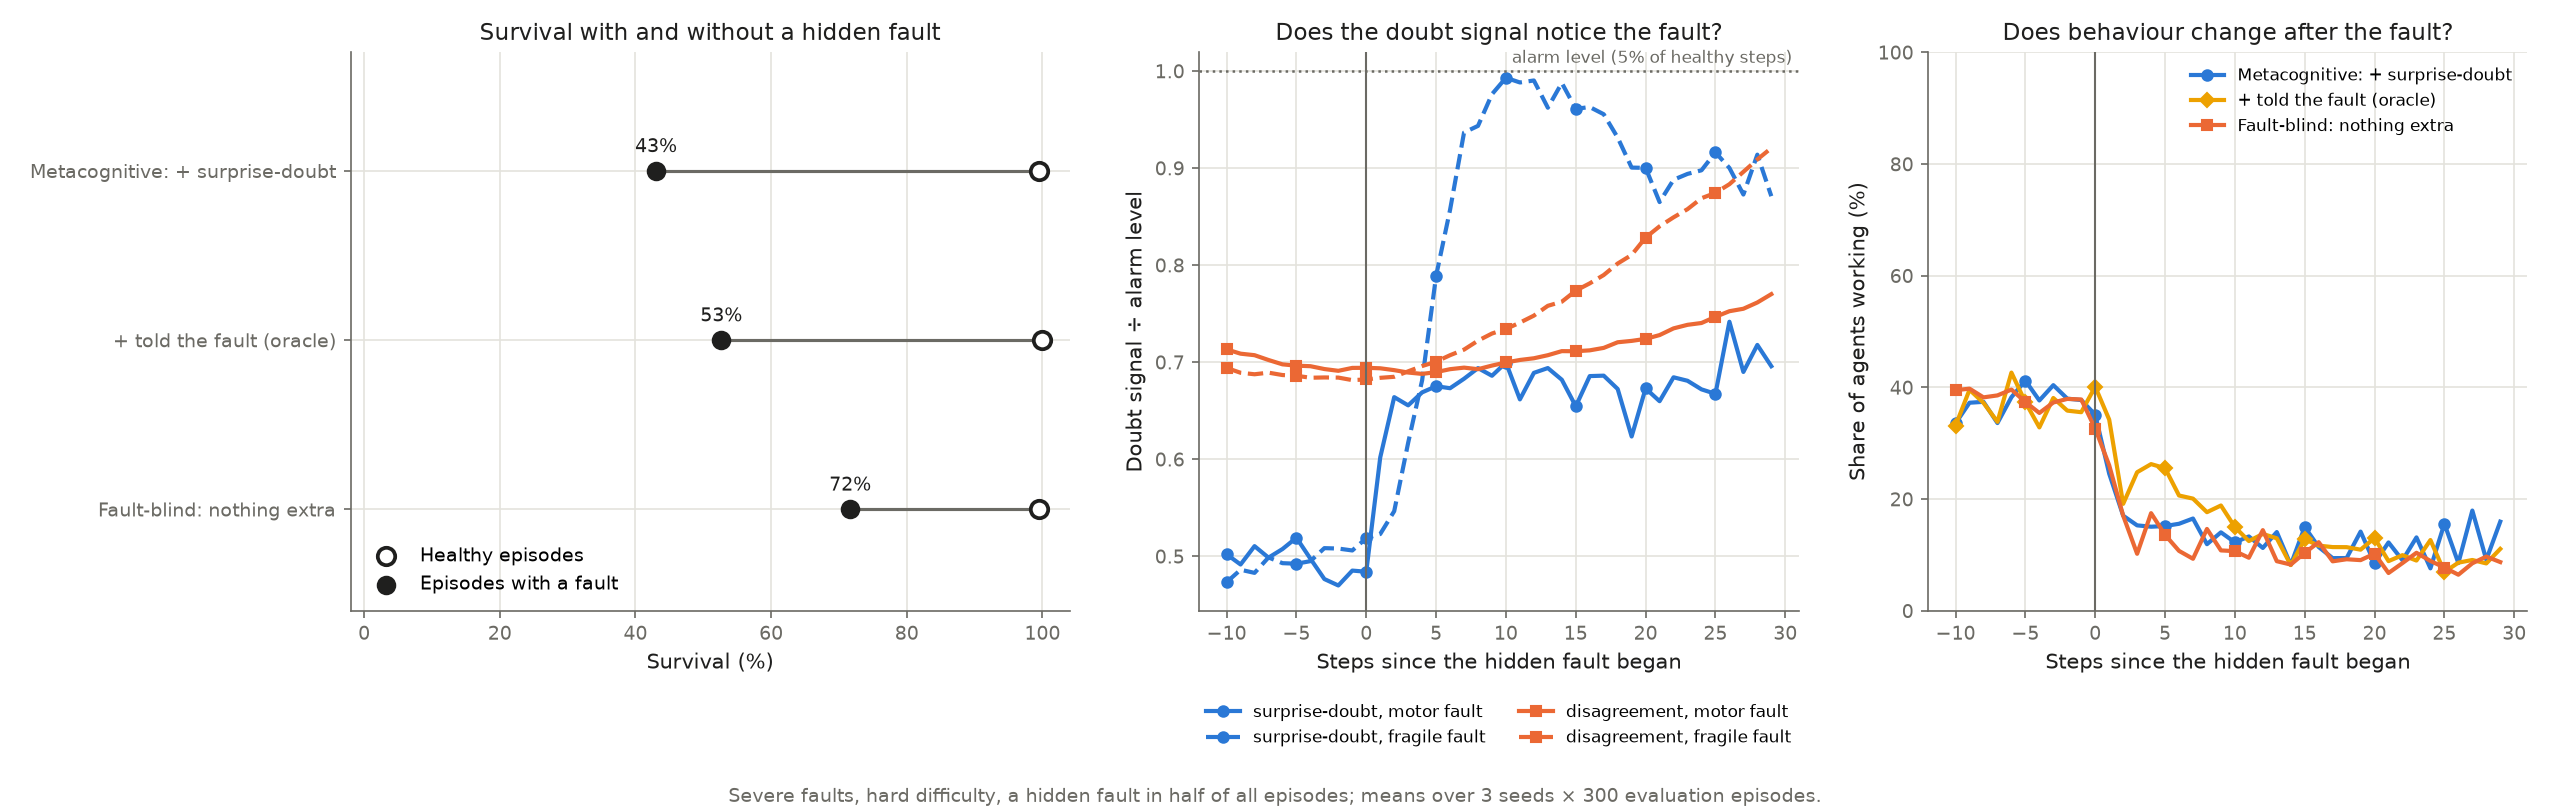
\includegraphics[width=\linewidth]{figures/fault_results_severe.png}
\caption{Severe hidden faults (from the research branch). Left: survival. Middle: surprise-doubt rises sharply
after onset of a fragile fault and moderately after a motor fault; ensemble disagreement drifts slowly. Right:
all agents reduce work similarly after a fault, whether or not they detect it.}
\label{fig:faults}
\end{figure}

\subsection{Evolved organisms and rules-only genomes}
\label{sec:organisms}
The metacognitive loop was then moved inside one small network trained by evolution only (OpenAI-ES
\citep{salimans2017evolution}; 400 generations, population 128, 32 lives per genome per generation; test: 600
new lives). Plastic weights are $W+A\odot H$, with $H$ updated during life by a three-factor rule
(pre $\times$ post $\times$ neuromodulator); a readout predicts resource and damage changes and learns during life
by the delta rule; doubt is a running average of its error and is fed back as input; a neuromodulator unit reads
doubt and gates plasticity. The \emph{rules-only} organism inherits no weights: each life starts from random
wiring and an empty self-model, and the genome holds only per-neuron learning-rule coefficients (161 numbers).

\begin{table}[t]
\centering\small
\caption{Evolved organisms, severe faults, hard difficulty. Per-seed healthy / fault survival (\%) on 600 test
lives. A run ``succeeds'' if healthy survival exceeds 90\pct. Source: \texttt{results/organism\_severe/*.json}.}
\label{tab:organisms}
\begin{tabular}{lrcccc}
\toprule
Organism & Genome & Seed 0 & Seed 1 & Seed 2 & Successes\\
\midrule
Innate wiring & 288 & 14.2 / 5.9 & 0.0 / 0.0 & 99.0 / 72.1 & 1/3\\
Innate + told the fault & 320 & 8.8 / 7.9 & 99.3 / 74.7 & 97.2 / 73.4 & 2/3\\
Innate + self-model and doubt & 736 & 99.7 / 68.4 & 100.0 / 73.0 & 99.7 / 73.4 & 3/3\\
Plastic wiring, no doubt & 583 & 8.4 / 0.0 & 100.0 / 65.8 & 97.6 / 73.7 & 2/3\\
Full organism (doubt gates plasticity) & 1095 & 99.3 / 67.4 & 100.0 / 71.7 & 100.0 / 68.6 & 3/3\\
Rules only (random wiring at birth) & 161 & 67.6 / 0.0 & 85.1 / 0.7 & 97.6 / 48.1 & 1/3\\
\bottomrule
\end{tabular}
\end{table}

\paragraph{Findings.}
\Sug\ All six runs of the two self-model-and-doubt families succeeded, versus 5 of 9 runs of the three
comparison families with inherited or plastic wiring (one-sided Fisher exact test, $p=0.092$; we recomputed this).
Three caveats bound this claim. (i) With three seeds per family, the test is underpowered. (ii) Genome size is
confounded: the doubt families have larger genomes (736 and 1095 vs.\ 288--583 parameters). (iii) The
\emph{successful} comparison runs reach the same level as the doubt families (e.g.\ innate seed 2: 99.0 / 72.1;
plastic seed 2: 97.6 / 73.7). The effect, if real, is on the \emph{reliability} of evolution, not on the
attainable level of performance.
\Neg\ In the full organism the evolved neuromodulator barely responds to faults (Figure~\ref{fig:organisms},
right): evolution used doubt as an input for action selection, not as a signal to rewire.
\Sug\ The rules-only organism can work: one of three runs reached 97.6\pct\ healthy survival from random wiring,
using only inherited learning rules. The same run survived only 48.1\pct\ of faulty lives, and the other two runs
did not succeed. This is a proof of possibility, consistent with \citet{najarro2020meta}, not evidence of
robustness.

\begin{figure}[t]
\centering
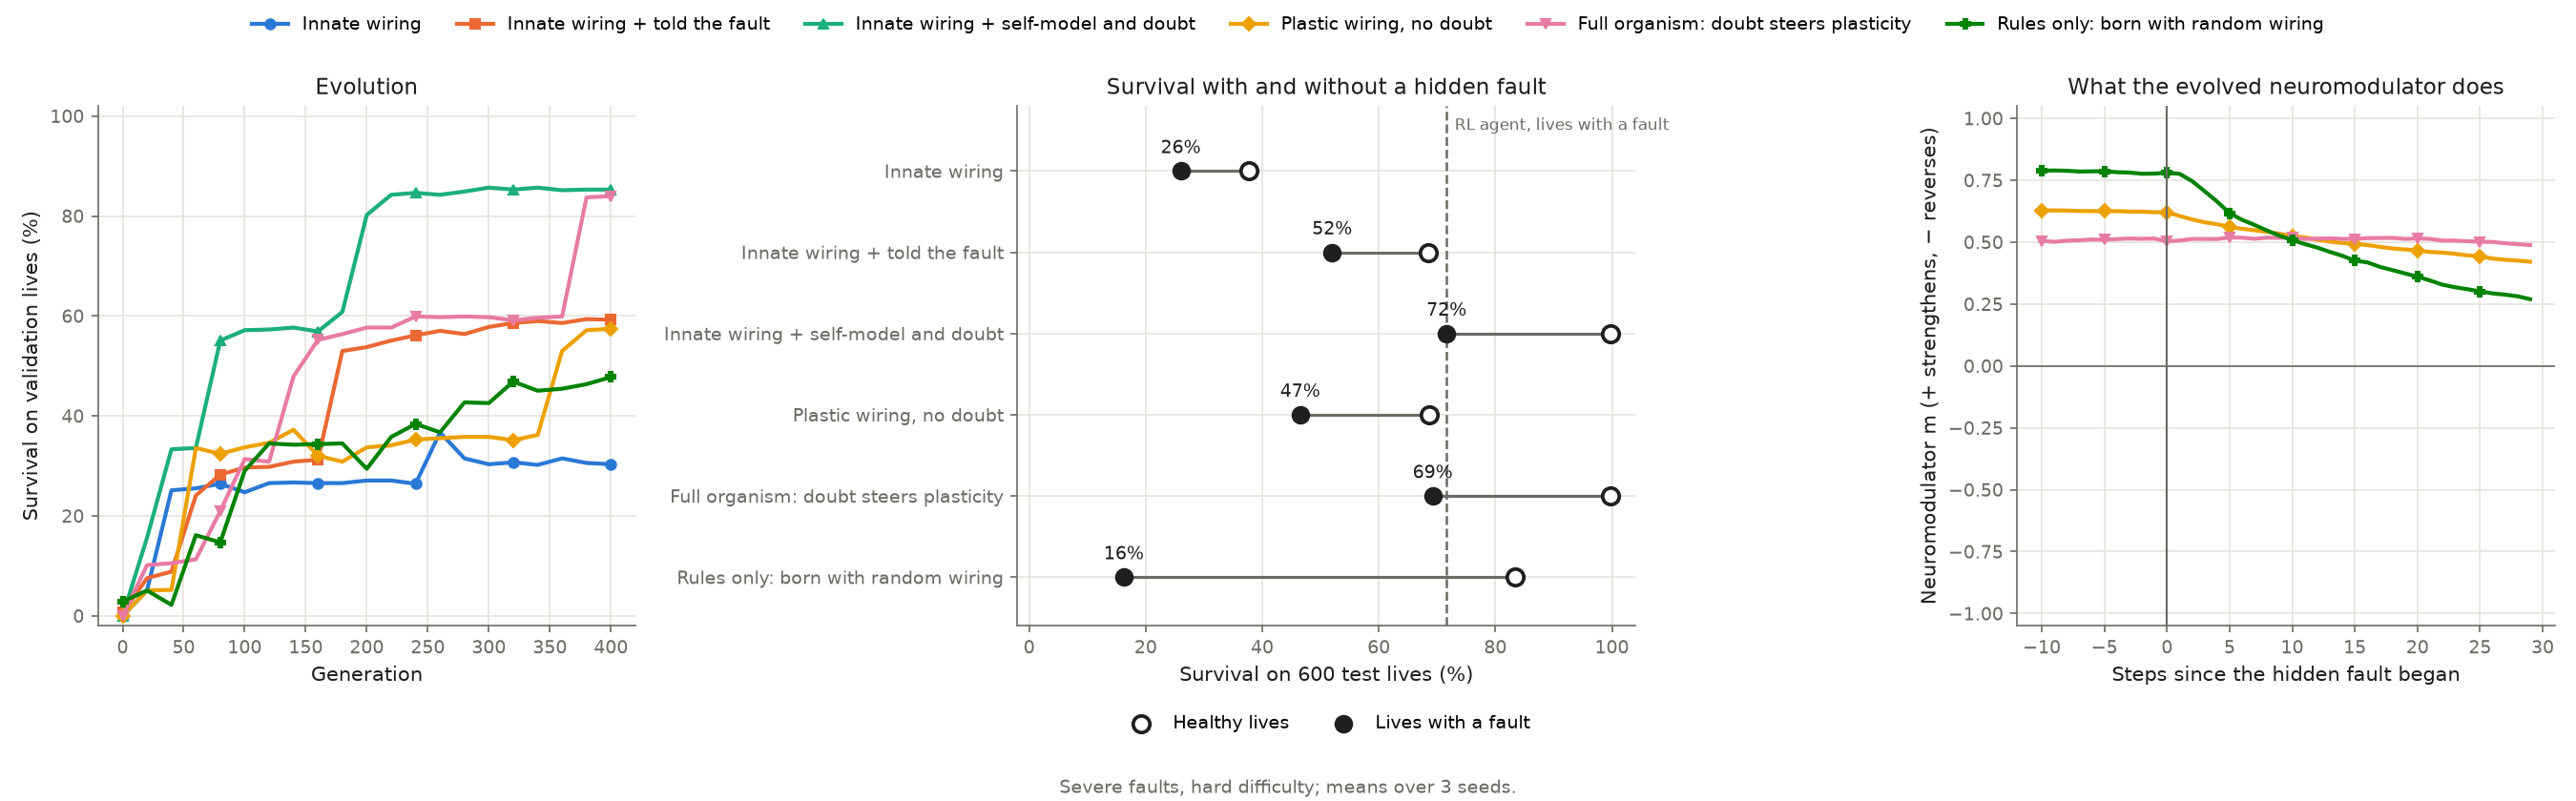
\includegraphics[width=\linewidth]{figures/organism_results.png}
\caption{Evolved organisms (research branch). Left: validation survival during evolution (seed means).
Middle: healthy vs.\ faulty test lives. Right: the evolved neuromodulator after fault onset---roughly flat in
the full organism.}
\label{fig:organisms}
\end{figure}

\subsection{The benchmark ceiling and the role of reward}
A dynamic-programming analysis over the known body dynamics (\path{survival_ceiling.py}, re-run for this paper)
gives the best survival any policy could reach once a severe fault strikes, even with instant knowledge of the
fault and full health at onset: 100.0\pct\ for the motor fault, 72.4\pct\ for the fragile fault, 86.2\pct\ overall.
\Dem\ The best agents already reach ${\approx}100\pct$ on the motor fault; all headroom is in the fragile fault,
where the best agents reach 39--47\pct\ (organisms) and 45\pct\ (fault-blind RL). Surviving a fragile fault
requires stopping work entirely, and the reward makes continued work worth the risk. Two lessons follow and
shaped everything after: a benchmark ceiling must be computed before an intelligence gain is claimed, and
self-knowledge cannot rescue an agent from an objective that rewards the behaviour that kills it.

%=====================================================================
\section{Part II --- Anchoring: why self-evaluation needs an external reference}
\label{sec:anchor}
%=====================================================================

Two failures in this program have the same structure. In Benchmark~B V2, ``learnability'' was defined from
changes in the self-model's own prediction error, and it could rise while behavioural accuracy fell
(\Rep; Section~\ref{sec:v1v3}). And the earlier write-ups of the original agent evaluated it with statistics
it partly generated itself. A companion note proposed a general principle, the Minimal Reference Condition
(MRC). We restate it, give a proof for a linear case (the original note gave none), and test it.

\subsection{Setting}
\begin{definition}[Self-modifying evaluator]
A system has parameters $\theta_t$ and an internal evaluator $E_t$. It updates $\theta$ to increase $E_t$ and
may also update $E_t$. True performance $T$ is fixed and not directly observed. The \emph{reference gap} is
any measure of divergence between $E_t$ and $T$; in the linear case $E_t(\theta)=w_t^\top\theta$,
$T(\theta)=v^\top\theta$, it is the angle $\Delta_t=\angle(w_t,v)$.
\end{definition}

\begin{proposition}[No guarantee without a reference]
If the evaluator update may select any $E_{t+1}$ from a class containing, for every value $c$, a function
equal to $c$ at $\theta_{t+1}$ regardless of $T(\theta_{t+1})$, then no rule that accepts updates by the
criterion $E_{t+1}(\theta_{t+1})>E_t(\theta_t)$ can guarantee $T(\theta_{t+1})\ge T(\theta_t)$.
\end{proposition}
\begin{proof}
Take any $\theta'$ with $T(\theta')<T(\theta_t)$ and choose $E'$ from the class with
$E'(\theta')=E_t(\theta_t)+1$. The pair $(\theta',E')$ satisfies the acceptance criterion and decreases $T$.
\end{proof}
\begin{remark}
The proposition is close to a tautology; its value is in naming the assumption that must be broken. It is an
instance of Goodhart's law \citep{goodhart1975problems,manheim2018categorizing} and of reward tampering
\citep{everitt2021reward}, specialized to an agent that can rewrite its own evaluator.
\end{remark}

\begin{definition}[Minimal Reference Condition, linear form]
A fixed unit vector $R$ with $\angle(R,v)\le\delta$ exists and every evaluator is projected onto the cone
$C(R,\epsilon)=\{w:\angle(w,R)\le\epsilon\}$ after each update.
\end{definition}

\begin{proposition}[Sufficiency of MRC for expected improvement, linear case]
Let $\theta_{t+1}=\theta_t+\eta P\hat w_t+\xi_t$ with $\hat w_t=w_t/\lVert w_t\rVert$, $\eta>0$, zero-mean
noise $\xi_t$, and a symmetric positive semi-definite preconditioner $P$ with $Pv=v$. Under MRC with
$\epsilon+\delta<\pi/2$,
\[
\mathbb E\big[T(\theta_{t+1})-T(\theta_t)\,\big|\,\theta_t,w_t\big]\;\ge\;\eta\cos(\epsilon+\delta)\;>\;0,
\qquad\text{so}\qquad \mathbb E[T(\theta_t)]\ge T(\theta_0)+\eta\,t\cos(\epsilon+\delta).
\]
\end{proposition}
\begin{proof}
$\mathbb E[T(\theta_{t+1})-T(\theta_t)]=\eta\,v^\top P\hat w_t=\eta\,(Pv)^\top\hat w_t=\eta\,v^\top\hat w_t=\eta\cos\angle(w_t,v)$.
By the triangle inequality for angles, $\angle(w_t,v)\le\angle(w_t,R)+\angle(R,v)\le\epsilon+\delta<\pi/2$, and
cosine is decreasing on $[0,\pi]$. Summing over $t$ gives the second statement.
\end{proof}
The condition $Pv=v$ allows the policy to move much more easily in directions orthogonal to $v$---cheap,
``cosmetic'' directions---without breaking the guarantee, because the anchored evaluator never rewards them
enough to dominate.

\subsection{Simulation}
We simulate the linear model ($n=20$, 400 steps, $\eta=0.05$, noise $\sigma=0.1$, 200 seeds;
\path{mrc_toy.py}). The evaluator self-endorses: $w\leftarrow w+0.05\,\hat\theta$. We run an isotropic policy
($P=I$) and a policy with a cheap direction $h\perp v$ ($P=I+9hh^\top$).

\begin{figure}[t]
\centering
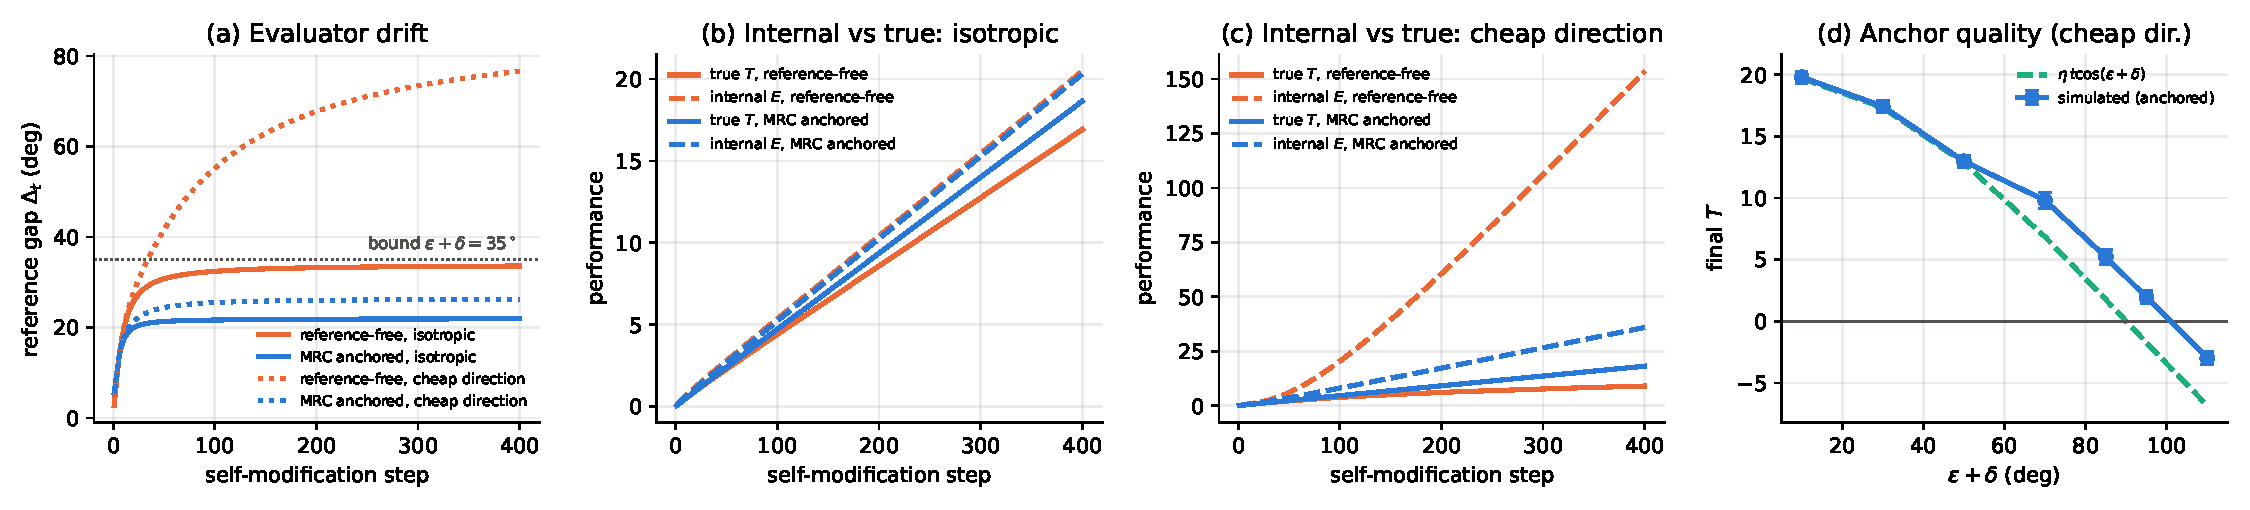
\includegraphics[width=\linewidth]{figures/mrc_toy.pdf}
\caption{Linear model of evaluator drift (200 seeds). (a) Reference gap. (b, c) Internal score $E$ (dashed) vs.\
true performance $T$ (solid). (d) Final $T$ under MRC as the anchor loosens, against the lower bound of
Proposition~2.}
\label{fig:mrc}
\end{figure}

\paragraph{Findings.} \Dem\ (for the model; this is a toy, not evidence about real systems.)
Without a cheap direction, the reference-free evaluator drifts to a gap of $33.6^\circ\pm5.4^\circ$ but true
performance still rises (final $T=16.9$ vs.\ 18.7 anchored): drift alone does not produce collapse, correcting a
claim in the original note. With a cheap direction, the reference-free gap grows to $76.7^\circ\pm5.3^\circ$ and
the internal score inflates to 153.6 while true performance reaches only 9.0; the anchored system keeps the gap
at $26.2^\circ$ (max $31.7^\circ$, below the $35^\circ$ bound), with $T=18.1$. Across anchor quality, final $T$
stays above the bound of Proposition~2 (Figure~\ref{fig:mrc}d).

\subsection{Anchoring in a metacognitive agent}
\label{sec:anchor-agent}
\Hyp\ A metacognitive signal is useful only if part of what it is scored against is generated outside the agent's
own modelling machinery. Surprise-doubt compares predictions to measured bodily change, which the agent cannot
rewrite; V2's self-model-based learnability did not, and drifted; V3's behavioural learnability is anchored to
task outcomes.

\Dem\ The self-graded variants of the original agent test the simplest case (Table~\ref{tab:msra-audit}). In them,
the self-model's error for the externally measured variables (load, resources, degradation) is computed---and the
self-model trained---against its own prediction instead of the measured value; control still sees the true
state. The only change is therefore what the evaluator is anchored to. On hard difficulty, the prediction error
the agent uses stops carrying information about shocks (AUROC 0.51 and 0.46, versus 0.90 for both anchored
counterparts), caution almost never triggers in the full agent (0.7\pct\ of steps), and survival falls from
$76.7$ to $48.7\pm11.0\pct$ (full agent) and from $94.0$ to $8.7\pm9.9\pct$ (rule-free variant). This is the
reference gap of Section~\ref{sec:anchor} in its most direct form: a self-evaluation that is free to agree with
itself agrees with itself. Two caveats: the manipulation also changes the self-model's training targets, so the
collapse combines an uninformative doubt signal with a self-model that never learns the measured dynamics; and
the original agent's ``actual'' state vector is itself half self-generated ($c_t,g_t,\delta_t$ are the agent's own
variables), so even its anchored doubt mixes an anchored and an unanchored component.

%=====================================================================
\section{Part III --- Developmental Benchmark B}
\label{sec:partIII}
%=====================================================================

\subsection{Why a new benchmark}
The homeostasis task gives an agent no reason to grow: a 32-unit controller is enough, so a rational developmental
system should learn not to grow, and the absence of growth there falsifies nothing. Benchmark~B was designed so
that capacity could matter:
\begin{itemize}
  \item each life draws new random mappings $(q,c)\mapsto a^*$ from task $q$ and cue $c$ to action, so the genome
        cannot memorize them and must encode \emph{how to learn} them (default 4 tasks $\times$ 4 cues $\times$
        4 actions; chance 25\pct);
  \item trials are delayed: task and cue are visible at an instruction step and hidden at the response step;
  \item tasks accumulate over four phases, with the newest task dominant and a rehearsal fraction of older tasks;
  \item hidden body faults can occur, and there is an energy/damage economy;
  \item the organism starts small and may grow or prune units; lifetime learning is local (no backpropagation);
        evolution (ES) tunes the genome.
\end{itemize}

\subsection{Benchmark integrity audit}
\label{sec:integrity}
Accuracy above 25\pct\ is not evidence of associative learning. We audited the benchmark code for shortcuts;
Table~\ref{tab:integrity} lists what we found.

\begin{table}[t]
\centering\small
\caption{Shortcut and integrity audit of Benchmark~B (V3/V4 code).}
\label{tab:integrity}
\begin{tabularx}{\linewidth}{>{\raggedright\arraybackslash}p{3.3cm}>{\raggedright\arraybackslash}p{4.2cm}X}
\toprule
Risk & Present? & Consequence and remedy \\
\midrule
Class imbalance within a phase & Yes. Four cues map to four actions independently, so collisions are common;
the best constant action per phase scores $\approx$50\pct. & Any learner can exceed chance by learning a phase
action prior. Report the cue-blind margin, not accuracy vs.\ chance. \\
Time / phase observable & Yes. Normalized time $t/(T-1)$ is an input, so phase identity is decodable. &
Phase-conditioned priors are learnable. The hindsight per-phase cue-blind baseline covers this; an online
cue-blind learner with the time input should also be run. \\
Task-frequency prior & Yes. The newest task gets 70\pct\ of trials (V4 meta test: 50\pct). & Favours recency;
report per-task retention (\texttt{task0} columns). \\
Reward leakage & Previous trial's perceived reward is visible at the next instruction. & Enables
win-stay/lose-shift across trials; cues are re-drawn every trial, so this helps only as a prior. Keep, but
ablate. \\
Action-dependent cost & Yes. Energy cost rises with the action index. & Survival pressure favours low-index
actions independently of the cue; fitness can conflict with accuracy. Report accuracy separately from fitness. \\
Fault leakage & Faults act through visible energy/damage. & Legitimate: detecting a fault from its bodily
effects is the point. \\
Hindsight baseline & The cue-blind phase baseline chooses the best action per phase \emph{in hindsight}. & It is
an upper bound on cue-blind strategies with phase knowledge, not an online agent; margins above it are
conservative. \\
Degenerate control & In V4 the no-plasticity control is bit-identical to random policy (zero readout $\to$
uniform policy, same random stream). & It does not test birth wiring in V4; V3's no-plasticity control (25.3\pct)
does. \\
Delay length & One recurrent step between instruction and response. & A short delay: memory is barely tested. \\
\bottomrule
\end{tabularx}
\end{table}

\subsection{V1--V3: dense local learners fail to learn the mapping}
\label{sec:v1v3}
All numbers in this subsection are \Rep\ (research log \path{docs/RESULTS.md} and the project draft; GPU runs;
no committed per-run result files).

\paragraph{V1.} Random birth wiring, recurrent state, local plastic weights, self-model, doubt, a learnability
estimate, and HOLD/GROW/PRUNE decisions with reserve neurons. With six actions (chance 16.7\pct), accuracy stayed at
16--17\pct\ from generation 0 to 50 while the phenotype underwent ${\approx}35$ structural changes per life and
drifted toward ${\approx}10$ neurons. \Neg\ Structural change without a working learner is noise. Diagnosis: no
reliable lifetime learner; lethal cognitive errors; structural decisions far too frequent; delayed reward not
credited to the instruction-time state.

\paragraph{V2.} Four cues and actions (chance 25\pct), eligibility traces across the delay, reward-gated
three-factor plasticity, stochastic softmax responses, a rehearsal curriculum, non-lethal cognitive errors, a
slower structural clock, and a genome seeded near a reward-modulated Hebbian rule. Final evaluation: 35.5\pct\
accuracy (phases 39.7 / 35.2 / 34.1 / 33.1\pct), 99.5\pct\ survival, a within-life rise from ${\approx}28\pct$ to
${\approx}40\pct$ followed by decline as tasks accumulated, and essentially no growth (16.0 average neurons;
0.26 structural changes per life). \Neg\ No developmental growth.

\paragraph{V3.} Per-trial eligibility reset (V2's traces credited ${\approx}72\pct$ of each reward to earlier
trials with different cues), reward-prediction-error neuromodulation, an $\text{onehot}(a)-\pi$ output rule,
evolvable temperature, recurrent gain normalization, stronger cue input, behavioural learnability and capacity
pressure. Controls: random policy 25.06\pct; no plasticity 25.34\pct. Fixed-16 evolution (100 generations):
37.7\pct\ at generation 0, 39.3\pct\ final (survival 99.7\pct). Cue-blind lifetime baseline 39.9\pct; cue-blind
per-phase baseline 49.7\pct; perfect-learner ceiling ${\approx}82\pct$. The within-life trace rose during phase 1
(30.3 $\to$ 38.5 $\to$ 44.2 $\to$ 51.7\pct) and dropped to 39.8\pct\ at the start of phase 2.
\Neg\ $39.3\pct<49.7\pct$: the V3 learner did not demonstrate $(q,c)\mapsto a$ learning; its behaviour is
consistent with learning a phase-dependent action prior that is overwritten when the task distribution
changes.

\paragraph{V3 diagnostics.} \Rep\ (hand-built rule, 200 lives; \path{docs/RESULTS.md}). A per-life ridge probe on
response-time states decoded the \emph{cue} at 93.9\pct\ (baseline 24\pct) and the task$\times$cue conjunction at
63.4\pct\ (baseline 8.9\pct), while the organism scored 37.6\pct\ against a 49.5\pct\ cue-blind baseline. Removing the
delay (cue visible at response) raised accuracy only to 40.6--43.7\pct\ (probe ${\approx}98\pct$ / ${\approx}71\pct$);
leaky units lowered it to 34.3\pct; a centered readout gave 40.2\pct. Interpretation: retention across the one-step
delay is not the main bottleneck; the information is largely present, but dense reward-modulated updates of
shared weights cannot bind 16 conjunctions from ${\approx}7$ exposures each without mutual overwriting. These
diagnostics are single-configuration runs without seed statistics.

\paragraph{Learnability in V3.} Behavioural learnability (a fast-minus-slow accuracy trend predicted from the
organism's features) was reported to rise while accuracy improved (${\approx}{+}0.42$ at 51.7\pct\ accuracy) and fall
below zero (${\approx}{-}0.10$) after task transitions, while capacity pressure rose. We test the prospective
version of this claim in Section~\ref{sec:learnability}.

\subsection{V4: a sparse associative learner and functional growth}
\label{sec:v4}
The V3 diagnosis---information present, dense readout interfering---led to V4
(\path{dsm_benchmark_b_v4.py}): the instruction's task+cue input is projected through random birth wiring to a
pool of 128 potential units, of which the active ones compete in a $k$-winners-take-all code ($k=1$); the code is
held across the delay and read out by a fast associative matrix trained with the same local three-factor rule,
$\Delta W=\eta\,m_t\,z\,(\text{onehot}(a)-\pi)^\top$, with $m_t$ driven by reward-prediction error (and optionally
doubt and learnability). \emph{Imprint growth} recruits a dormant unit whose input weights are set to the current
pattern, when the controller decides to grow and no active unit already owns that pattern (novelty gate);
\emph{random growth} recruits a dormant unit with its random birth wiring. The configurations
\emph{full}, \emph{nolearn} and \emph{basic} use imprint growth plus pruning; \emph{nolearn} removes learnability
and \emph{basic} removes all self-model signals from the controller, gate and modulator.

All V4 results below use a \emph{hand-specified} genome---no evolution---and were re-run for this paper on CPU:
3 seeds $\times$ 400 lives (standard task) or 200 lives (metacognition test), every configuration on the same
lives. Standard task: 4 tasks $\times$ 4 cues $\times$ 4 actions, 240 steps, faults in 65\pct\ of lives.

\begin{table}[t]
\centering\footnotesize\setlength{\tabcolsep}{4pt}
\caption{V4, standard task, hand-built genome (mean $\pm$ SD over 3 seeds; each seed 400 paired lives). Cue-blind =
best constant action per phase in hindsight (50.0\pct); perfect-learner ceiling 80.4\pct\ (seed 0).
Source: \texttt{paper/results/v4\_standard/}.}
\label{tab:v4}
\begin{tabular}{lcccccc}
\toprule
Configuration & Accuracy & Margin & Task 0, ph.\ 4 & Avg.\ units & Final units & Grows\\
\midrule
Random policy & $24.9\pm0.1$ & $-25.1$ & 24.8 & 16 & 16 & 0\\
Fixed-8 & $46.3\pm0.2$ & $-3.7$ & 67.0 & 8 & 8 & 0\\
Fixed-16 & $50.5\pm0.2$ & $+0.5$ & 74.4 & 16 & 16 & 0\\
Fixed-32 & $53.8\pm0.1$ & $+3.8$ & 77.7 & 32 & 32 & 0\\
Fixed-64 & $56.7\pm0.3$ & $+6.7$ & 83.4 & 64 & 64 & 0\\
Fixed-128 & $58.6\pm0.3$ & $+8.6$ & 86.0 & 128 & 128 & 0\\
\midrule
Random-wired growth from 16 & $50.5\pm0.0$ & $+0.5$ & 56.0 & 41.8 & 67.8 & 51.8\\
Imprint growth from 16 & $58.6\pm0.6$ & $+8.6$ & 87.5 & 23.9 & 29.8 & 13.8\\
Full (imprint + prune) & $58.4\pm0.6$ & $+8.4$ & 87.4 & 23.9 & 29.6 & 13.9\\
Full without learnability & $58.6\pm0.5$ & $+8.6$ & 87.5 & 24.0 & 29.7 & 14.0\\
Full without self-model signals & $56.4\pm0.4$ & $+6.4$ & 83.5 & 23.4 & 29.0 & 13.2\\
\bottomrule
\end{tabular}
\end{table}

\begin{figure}[t]
\centering
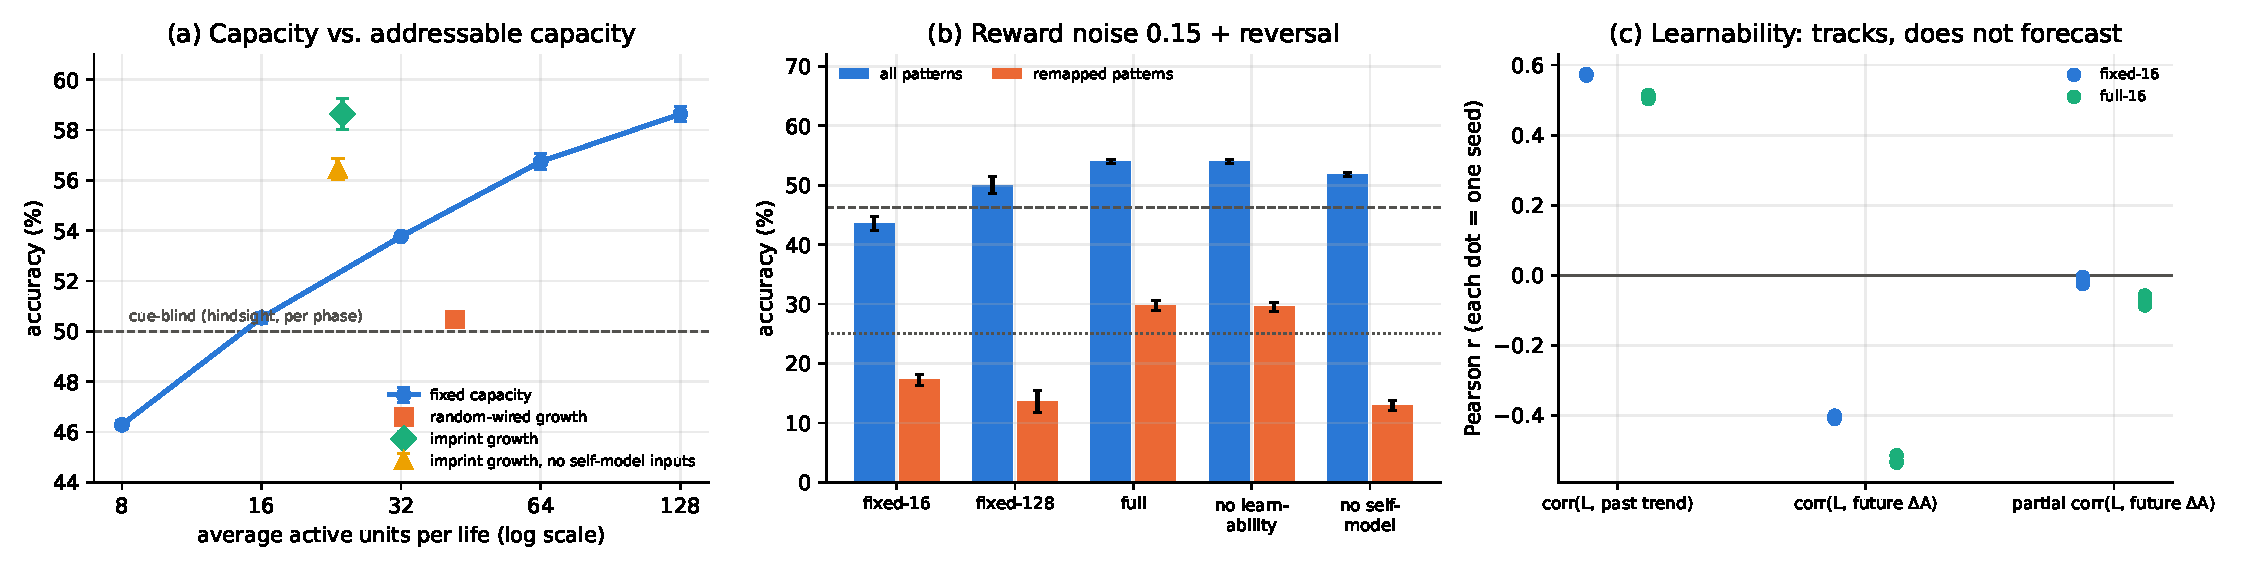
\includegraphics[width=\linewidth]{figures/v4_results.pdf}
\caption{V4 (hand-built genome, 3 seeds). (a) Accuracy vs.\ average active units: fixed capacity (line), random-wired
growth, imprint growth, and imprint growth without self-model inputs. Dashed: hindsight cue-blind baseline.
(b) Reward noise 0.15 plus mid-life remapping of two tasks: overall accuracy and accuracy on remapped patterns.
Dashed: cue-blind; dotted: chance. (c) Learnability validation (Section~\ref{sec:learnability}).}
\label{fig:v4}
\end{figure}

\paragraph{Findings.}
\begin{enumerate}[leftmargin=*]
  \item \Dem\ \textbf{Capacity matters in this learner.} Accuracy rises monotonically with fixed size
        (46.3 $\to$ 58.6\pct\ from 8 to 128 units; seed SD $\le0.3$). This is the precondition that made growth
        worth studying, and it did not hold for the dense learners.
  \item \Dem\ \textbf{Addressability, not unit count.} Random-wired growth uses on average 18 more units than
        imprint growth yet gives no improvement over fixed-16 (50.5 vs.\ 50.5\pct), and worse retention of task 0
        (56.0 vs.\ 74.4\pct). Imprint growth reaches the fixed-128 level (58.6 vs.\ 58.6\pct) with 23.9 average units,
        and the best task-0 retention (87.5\pct). The per-seed differences imprint $-$ random are $+8.0$, $+8.9$ and
        $+7.7$ points on identical lives.
  \item \Neg\ \textbf{Metacognition is not what drives growth here.} Removing learnability changes nothing
        (58.6 vs.\ 58.4\pct); removing all self-model signals costs 2.0 points. GROW decisions occur at slightly
        \emph{lower} capacity pressure than HOLD decisions after an error (difference $-0.032$ to $-0.036$ across
        seeds): the novelty gate, not pressure, decides. In the standard task every error signals ``this pattern
        has no slot yet'', so novelty is a sufficient trigger.
  \item \Neg\ \textbf{Even fixed-16 in V4 does not clear the cue-blind baseline} ($+0.5$ points). Capacity-limited
        sparse learning is still close to the shortcut regime; only larger or growing networks clear it by a
        margin (${\approx}8.5$ points), which is still far below the 80.4\pct\ ceiling.
\end{enumerate}
The imprint rule is, in essence, a resource-allocating network \citep{platt1991resource} with a local
three-factor readout: its success confirms an old idea in a new setting rather than establishing a new mechanism.

\paragraph{Evolved genomes.} \Sug\ The repository also contains V4 runs in which ES tuned the genome (population 64,
32 lives per genome, 100 generations; the 53-parameter genome without repair and gate genes). Table~\ref{tab:v4evo}
lists every committed run. Evolution raised every configuration (fixed-16 from 50.5 to 54.2\pct, now 4.5 points above
cue-blind), and the ordering of Table~\ref{tab:v4} is preserved: imprint growth (67.1\pct, 23.9 average units)
exceeds fixed-128 (64.5\pct), random growth stays near fixed-16 (54.8\pct), and imprint accuracy \emph{rises} across
phases (62.7 $\to$ 69.1\pct) where fixed networks decline (fixed-128: 70.4 $\to$ 60.6\pct). With one seed for every
growth configuration, these are suggestive only: seed-to-seed spread in the two-seed rows is ${\le}0.9$ points, but a
single evolutionary run can differ from another in ways the evaluation spread does not capture. Evolved
\emph{full}, \emph{nolearn} and \emph{basic} are indistinguishable (67.0, 66.8, 67.1\pct), confirming that
self-model signals are redundant in the standard task.

\begin{table}[t]
\centering\footnotesize\setlength{\tabcolsep}{4pt}
\caption{V4, evolved genomes (ES, 100 generations), standard task. One row per committed run. Cue-blind
49.7--49.8\pct; survival 99.7--100\pct\ in every run; random-growth units are the mean of the two seeds. Source: \texttt{results/v4\_standard/*\_seed*.json} in the developmental-self-model repository.}
\label{tab:v4evo}
\begin{tabular}{lcccc}
\toprule
Configuration (seeds) & Accuracy & Avg / final units & Phase 1 $\to$ 4 (seed 0) & Task 0, ph.\ 4\\
\midrule
Fixed-16 (0, 1) & 54.2 / 54.2 & 16 / 16 & 63.9 $\to$ 46.4 & 75.2 / 73.3\\
Fixed-32 (0, 1) & 58.7 / 58.6 & 32 / 32 & 67.1 $\to$ 51.8 & 79.5 / 79.3\\
Fixed-64 (0, 1) & 62.5 / 61.6 & 64 / 64 & 69.6 $\to$ 56.7 & 84.0 / 83.6\\
Fixed-128 (0, 1) & 64.8 / 64.2 & 128 / 128 & 70.9 $\to$ 60.4 & 86.4 / 86.0\\
Random growth (0, 1) & 55.0 / 54.6 & 38.7 / 62.8 & 62.2 $\to$ 49.8 & 57.7 / 59.5\\
Imprint growth (0) & 67.1 & 23.9 / 29.6 & 62.7 $\to$ 69.1 & 85.7\\
Full (0) & 67.0 & 23.9 / 29.6 & 62.6 $\to$ 68.7 & 85.6\\
Full without learnability (0) & 66.8 & 23.9 / 29.5 & 62.5 $\to$ 68.6 & 84.9\\
Full without self-model signals (0) & 67.1 & 23.7 / 29.4 & 62.9 $\to$ 68.9 & 85.4\\
\bottomrule
\end{tabular}
\end{table}

\paragraph{Metacognition under ambiguous errors.}
To create conditions in which an error is \emph{not} always a missing slot, V4.1 adds reward noise (15\pct\ of
feedback flipped; fitness scores the true outcome) and a mid-life remapping of two tasks, plus a REPAIR action
that resets the slot owning the current pattern, with a hand-set connection from a per-slot surprise signal
(``slot doubt'': recent confident-error rate of that unit) to REPAIR and to a plasticity gate (480 steps,
rehearsal 0.5, no faults).

\begin{table}[t]
\centering\footnotesize\setlength{\tabcolsep}{4pt}
\caption{V4.1, reward noise 0.15 + reversal, hand-built genome (3 seeds $\times$ 200 paired lives).
Cue-blind 46.2\pct; ceiling 90.0\pct. Source: \texttt{paper/results/v4\_meta/}.}
\label{tab:v4meta}
\begin{tabular}{lccccc}
\toprule
Configuration & Accuracy & Remapped & Task 0, ph.\ 4 & Avg.\ units & Repairs/life\\
\midrule
Random policy & $25.2\pm0.2$ & 25.1 & 23.8 & 16 & 0\\
Fixed-16 & $43.5\pm1.1$ & $17.2\pm0.9$ & 15.3 & 16 & 0\\
Fixed-128 & $50.0\pm1.5$ & $13.6\pm1.8$ & 11.8 & 128 & 0\\
Full-16 & $53.9\pm0.3$ & $29.8\pm0.9$ & 36.9 & 24.8 & 18.8\\
Full-16 without learnability & $54.0\pm0.3$ & $29.5\pm0.8$ & 35.9 & 24.8 & 18.7\\
Full-16 without self-model signals & $51.7\pm0.3$ & $12.9\pm0.8$ & 8.8 & 24.4 & 0.3\\
\bottomrule
\end{tabular}
\end{table}

\Dem\ (hand-wired) A per-slot surprise signal lets the organism find and reset slots whose mapping changed:
accuracy on remapped patterns is 29.8\pct\ with it and 12.9\pct\ without it (paired lives, 3 seeds; per-seed
differences $+17.3$, $+16.3$, $+17.1$). Because the ablation removes the signal from REPAIR, from the gate and from
the modulator together, the effect cannot yet be assigned to one lever; and because the REPAIR connection was set
by hand, this shows that the signal is \emph{usable}, not that evolution would discover its use.
\Neg\ Again learnability contributes nothing (54.0 vs.\ 53.9\pct). Note also that all learners except the repairing
ones score \emph{below chance} on remapped patterns: they keep executing the old mapping.
\Neg\ The benefit depends on the condition. In a smaller per-condition check (\Rep; 40 lives $\times$ 3 seeds,
\path{docs/RESULTS.md}) full $-$ basic was $+1.9$ (standard), $-2.0$ (noise only), $+5.2$ (reversal only) and $+2.6$
points (noise + reversal): under noise alone, the hand-set repair policy fires on noise and hurts. Whether evolution
tunes this away is untested.

\subsection{Is the learnability signal a forecast? A pre-specified prospective test}
\label{sec:learnability}
The strongest version of Q3 is that the agent predicts its \emph{future} learning progress. The V3/V4
learnability signal $L_t$ is trained online to predict $\tanh(10(\bar a^{\text{fast}}_t-\bar a^{\text{slow}}_t))$,
a \emph{retrospective} trend of recent accuracy. We therefore tested it prospectively
(\path{learnability_validation.py}; criteria written in the script header before it was run). For each life
and response step $t$ with $W=10$: $\Delta A_t=\text{mean}(\text{correct}_{t+1..t+W})-\text{mean}(\text{correct}_{t-W+1..t})$.
Criteria: \textbf{S1} $\operatorname{corr}(L_t,\text{trend}_t)>0.3$ (tracks the past); \textbf{S2}
$\operatorname{corr}(L_t,\Delta A_t)>0$ with a life-level bootstrap 95\pct\ CI excluding 0 (forecasts); \textbf{S3}
the same for the partial correlation after regressing both on recent trend, $1-\bar a^{\text{slow}}$, past-window
accuracy and phase (adds information). All three had to hold in every seed. V4 hand-built genome, fixed-16 and
full-16, 3 seeds $\times$ 400 lives ($\approx$40{,}400 samples per run). In fixed-16, learnability is a passive
readout that does not affect behaviour, so the test has no feedback loop.

\begin{table}[t]
\centering\footnotesize\setlength{\tabcolsep}{4pt}
\caption{Prospective validation of learnability (seeds 0 / 1 / 2; 95\pct\ life-level bootstrap intervals in the source
file \texttt{paper/results/learnability\_validation.json}).}
\label{tab:learn}
\begin{tabular}{lcccc}
\toprule
Run & $r(L,\text{trend})$ [S1] & $r(L,\Delta A)$ [S2] & partial $r$ [S3] & $r(\text{tr.},\Delta A)$\\
\midrule
Fixed-16 & 0.575 / 0.570 / 0.572 & $-0.400$ / $-0.410$ / $-0.406$ & $-0.011$ / $-0.025$ / $-0.004$ & $-0.30$\\
Full-16 & 0.515 / 0.508 / 0.503 & $-0.513$ / $-0.531$ / $-0.535$ & $-0.057$ / $-0.072$ / $-0.086$ & $-0.35$\\
\bottomrule
\end{tabular}
\end{table}

\Neg\ \textbf{S1 passes; S2 and S3 fail in every run.} The signal tracks past progress, and it correlates
\emph{negatively} with future progress---a recent upswing predicts regression to the mean. After controlling
for trivial statistics its partial correlation with future progress is zero (fixed-16; all three bootstrap
intervals include 0) or slightly negative (full-16; intervals exclude 0 on the negative side). An event study
reproduces the qualitative V3 pattern---$L_t$ is highest just before a task transition (0.24 in fixed-16) and decays
to ${\approx}0$ within 14 responses---but the decay lags the accuracy drop, as a retrospective signal would.
\textbf{Consequence:} the claim ``the agent represents that its behaviour is improving'' is supported only in
the retrospective sense. This is not surprising given the training target; a forecasting version would have to
be trained on a delayed target (the realized $\Delta A$ once $t+W$ is reached), which is local and causal
(Section~\ref{sec:program}, E8).

\subsection{Why naive GROW-vs-HOLD comparisons mislead}
The V3/V4 code compares accuracy on the next occurrences of the same pattern after GROW vs.\ HOLD decisions.
In the V4 standard runs this gives 36--38\pct\ after GROW and 53--55\pct\ after HOLD (all seeds), which read naively
says growth \emph{hurts}. It does not: GROW is chosen on first encounters with a pattern (novelty gate), HOLD
mostly on patterns that already have a slot. The comparison is dominated by selection; the between-condition
comparison in Table~\ref{tab:v4} (same lives, growth enabled or not) is the valid causal estimate. A
decision-level causal estimate requires randomizing the structural action (E9).

%=====================================================================
\section{Reviewer-2 audit of this program's earlier claims}
\label{sec:audit}
%=====================================================================

Table~\ref{tab:audit} lists statements from earlier drafts and write-ups that do not survive scrutiny, and what
replaces them here. We include it because the project's credibility depends on it.

\begingroup\small
\begin{longtable}{>{\raggedright\arraybackslash}p{5.2cm}>{\raggedright\arraybackslash}p{4.6cm}>{\raggedright\arraybackslash}p{4.8cm}}
\caption{Audit of earlier claims.}\label{tab:audit}\\
\toprule
Earlier claim & Problem & Status here\\
\midrule\endfirsthead
\toprule Earlier claim & Problem & Status here\\ \midrule\endhead
MSRA: 100\pct\ survival vs.\ 67\pct\ (MBRL), 73\pct\ (PPO), 81\pct\ (fixed $\beta$), 86\pct\ (PPO-Lagrangian); ablation and
sensitivity tables; $t(29)=15.32$, Cohen's $d=2.41$ & No baseline, ablation or statistics code or output exists
in any branch. & Withdrawn. Replaced by the re-executed audit (Table~\ref{tab:msra-audit}). \\
MSRA's 100\pct\ survival demonstrates the value of metacognition & On normal difficulty always-rest also survives
100\pct; on expert the agent survives 5.3\pct. & Uninformative; the discriminating regime (hard) shows doubt helps
survival at a large reward cost. \\
MSRA switches to caution ``without explicit hard-coding'' & \path{select_action} applies hand-written
thresholds before metacognition; imagination is filtered by hard-coded environment costs. & False; corrected
(Section~\ref{sec:msra-audit}). \\
Doubt: $\gamma=0.95$, thresholds $0.15/0.05$; 5\pct\ shocks & Code: $0.7/0.3$ mixing, thresholds $0.02/0.005$;
the run configuration uses expert difficulty (15\pct\ shocks). & Replaced by the code's values (Eq.~\ref{eq:doubt}). \\
Doubt--$\beta$ correlation $R^2=0.89$ & $\beta$ is defined as a function of doubt; the correlation is true by
construction. & Removed. \\
Phase portrait, shock-response and long-horizon figures & Not produced by any committed code. & Removed. \\
Parameter counts: self-model 12{,}422, actor-critic 8{,}961 & Actual: 11{,}462 and 14{,}790. & Corrected. \\
MSRA spends 4.4\pct\ of steps in caution mode (figure and preprint) & \path{main.py}'s own training loop
gives 91.6\pct\ (normal) and 98.2\pct\ (hard) with the committed code and no-op stand-ins for the missing module. &
Not reproduced; reported as such. \\
Actor-critic ``policy'' & Trained but never selects actions; update can diverge to NaN. & Reported
(Table~\ref{tab:msra-audit}). \\
MRC: ``we prove'' the anchored gap stays bounded; ``feedback loop causes $w_t$ to rotate away'' & No proof was given;
in the isotropic model drift saturates and $T$ still rises. & Proof given for the linear case (Prop.~2); collapse
shown to require a cheap direction. \\
Self-model + doubt organisms ``evolved more consistently'' & $n=3$ per family, $p=0.092$; genome-size confound;
successful comparison runs reach the same level. & Kept as \Sug\ with all three caveats. \\
Rules-only reached ${\approx}98\pct$ & One of three seeds, 97.6\pct\ healthy, 48.1\pct\ with faults. & Kept as proof of
possibility with the full per-seed record. \\
V3 learnability shows the organism knows ``my behaviour is improving'' & Tested only retrospectively. &
Prospective test fails (Section~\ref{sec:learnability}). \\
Capacity pressure drives growth & In V4, GROW occurs at lower pressure than HOLD. & Growth is novelty-driven in
the tested setting. \\
V2 accuracy above chance indicates learning of the task & Cue-blind baseline not computed. & Reinterpreted via V3
controls as action-prior learning. \\
No-plasticity control validates birth wiring (V4) & Bit-identical to the random-policy control in V4. &
Valid only for V3. \\
\bottomrule
\end{longtable}
\endgroup

%=====================================================================
\section{Claims}
\label{sec:claims}
%=====================================================================

\paragraph{Level A --- supported now.}
\emph{In small synthetic benchmarks, (i) an online self-model's prediction error is informative about hidden bodily
change and is associated with more reliable evolution of successful controllers (suggestive; 6/6 vs.\ 5/9 runs,
$p=0.092$), although detection by itself did not improve survival; (ii) for lifetime structural growth, what
matters is whether new capacity is addressable: with a hand-specified sparse associative learner, imprinting new
units on unrepresented patterns matched a fixed network five times larger in average size, while equally
triggered growth of randomly wired units gave no benefit (3 seeds, paired lives; single evolved runs show the same
ordering at a higher level); (iii) the growth decisions in that result are driven by
novelty, not by metacognitive estimates; a per-unit surprise signal becomes useful for repairing remapped
associations when errors are ambiguous; (iv) the agent's behavioural learning-progress signal tracks past
progress but does not forecast future progress; and (v) a doubt signal is useful only while it is anchored to
measured outcomes: graded against the agent's own predictions, it loses its information about disturbances and the
agent's survival collapses.}

\paragraph{Level B --- within reach of one or two experiments.}
\emph{An organism can forecast its own near-future learning progress from local signals (E8), and structural
allocation triggered by that forecast (persistent error $\times$ low predicted progress $\times$ novelty or
interference) improves learning over matched HOLD and novelty-only controls under conditions where novelty alone
is insufficient (E9--E10), with the controller's use of these signals discovered by evolution rather than set by
hand.}

\paragraph{Level C --- the long-term DSM hypothesis.}
\Hyp\ \emph{An artificial learner can discover during its lifetime that its present way of representing an experience
prevents it from learning it, and respond by constructing the computational structure needed to learn it---with
the learning rules, the self-model and the structural policy all inherited as a compact genome.}

\paragraph{Verdict.} \textbf{Suitable now as a workshop, negative-results or diagnostic paper; requires a small
number of decisive experiments for a main-track claim.} The threshold is concrete: a main-track paper on
metacognitively driven development would need (a) a learnability signal that passes S2 and S3 of
Section~\ref{sec:learnability} in $\ge5$ seeds, and (b) a randomized structural intervention showing that
growth triggered by that signal beats novelty-only growth and matched HOLD in a condition where novelty is not
sufficient, with the controller evolved rather than hand-set. Neither exists yet. What exists---the audit, the
negative results, the addressability control and the anchoring analysis---is defensible now.

%=====================================================================
\section{A minimal decisive experimental program}
\label{sec:program}
%=====================================================================
\Pro\ All experiments use Benchmark~B (V4 code unless stated), paired lives across conditions, $\ge5$ seeds
(more where the effect is small), and a fixed evaluation set of 1{,}000 lives per seed. Success criteria are
stated before running. The general statistical plan: paired differences per seed; mean, SD and all per-seed values;
Cohen's $d_z$ on paired differences; two-sided paired $t$-test (or Wilcoxon signed-rank when $n<8$ makes
normality untestable) with Holm correction within each experiment; for per-step analyses, bootstrap over lives.
Stopping: each experiment runs its pre-set budget; no early stopping on results.

\begingroup\footnotesize
\setlength{\tabcolsep}{3pt}
\begin{longtable}{>{\raggedright\arraybackslash}p{1.6cm}>{\raggedright\arraybackslash}p{3.0cm}>{\raggedright\arraybackslash}p{3.1cm}>{\raggedright\arraybackslash}p{3.3cm}>{\raggedright\arraybackslash}p{3.8cm}}
\caption{Decisive experiments. IV: independent variable; DV: dependent variable.}\label{tab:program}\\
\toprule
Exp. & Hypothesis & IV / DV / controls & Support / falsify & Failure modes\\
\midrule\endfirsthead
\toprule Exp. & Hypothesis & IV / DV / controls & Support / falsify & Failure modes\\ \midrule\endhead
E1 Representation probe (V3 dense) \newline\emph{(partly done, 1 config.)} & Task$\times$cue is linearly decodable at response time. & IV: size 16/32/64, delay on/off. DV: ridge-probe accuracy per life (held-out trials), measurement only. Controls: probe on shuffled labels; probe on birth-state network. 5 seeds. & High probe + low accuracy $\Rightarrow$ readout/credit bottleneck (reported: cue 93.9\pct, task$\times$cue 63.4\pct). Low probe even without delay $\Rightarrow$ representation bottleneck. & Probe overfits (use held-out trials); decodable but not linearly separable by a local rule. \\
E2 No-delay \newline\emph{(partly done)} & Recurrent retention is not the main bottleneck. & IV: delay vs.\ cue visible at response. DV: accuracy, cue-blind margin. 5 seeds. & Large gain without delay $\Rightarrow$ retention bottleneck; small gain supports interference diagnosis. & Cue visibility adds input drive, not only memory; match input norms. \\
E3 Leaky retention \newline\emph{(partly done)} & A local leaky unit rescues delayed performance if retention matters. & IV: leak $r\in\{0,0.5,0.8\}$. DV: accuracy, probe accuracy. 5 seeds. & Improvement proportional to E2 gap. & Leak increases cross-trial interference. \\
E4 Oracle learner (GRU, backprop) & The benchmark is learnable at 16--64 units with the available exposure. & (a) Meta-trained GRU (RL$^2$ style \citep{duan2016rl2}) over many lives, learning within life in activations; (b) tabular ideal learner. DV: accuracy vs.\ 80.4\pct\ ceiling, cue-blind margin. 5 seeds. & GRU at $\ge$60\pct\ with 32 units $\Rightarrow$ capacity/exposure are adequate and local learners are the bottleneck. GRU near cue-blind $\Rightarrow$ redesign benchmark. & Meta-training budget too small; report training curves to saturation. \\
E5 Fast associative memory (no growth) & Sparse code + local readout beats cue-blind at fixed size. & Done hand-built (Table~\ref{tab:v4}) and evolved with 2 seeds (Table~\ref{tab:v4evo}). Remaining: $\ge$5 seeds. & Evolved fixed-32 $\ge$ cue-blind $+5$ points in all seeds. & Evolution degrades a good hand rule (compare to generation 0). \\
E6 Cue-blind baselines & Claimed mapping learners beat the strongest cue-blind learner. & Add an \emph{online} cue-blind learner that sees time and task but not cue; keep hindsight baseline. & Margin $>0$ over both, per seed. & Online baseline weaker than hindsight; report both. \\
E7 Capacity scaling & Performance increases with fixed capacity. & Done for hand-built V4 (8--128 monotone). Repeat with evolved genomes and the V3 dense learner. & Monotone increase in $\ge$4 of 5 seeds. & Flat curve $\Rightarrow$ capacity is not the target; growth has nothing to fix. \\
E8 Learnability forecast & A locally trained forecaster predicts future $\Delta A$. & IV: target = retrospective trend (current) vs.\ delayed realized $\Delta A$ (new). DV: S1--S3 of Section~\ref{sec:learnability}; calibration curve of $L$ vs.\ realized $\Delta A$; within-phase analysis. 5 seeds. & S2 and S3 pass in all seeds. Falsified if the delayed-target forecaster also has partial $r\le0$. & Predictability of $\Delta A$ is itself near zero (compute the ceiling with an offline regressor on the same features). \\
E9 Growth causal test & At matched eligible states, GROW improves subsequent learning and retention vs.\ HOLD. & Randomize the structural action at eligible decisions (error + novel pattern) with $p=0.5$; DV: accuracy on the next 3 occurrences of the pattern, old-task retention, learning speed. 5 seeds $\times$ 1{,}000 lives. & Positive average treatment effect with CI excluding 0; supports causal usefulness of growth. & Randomization changes capacity trajectory; also report whole-life effects. \\
E10 Growth ablations & Metacognitive triggers beat novelty-only triggers when novelty is insufficient. & Configs: fixed-small, fixed-large, random growth, raw-error trigger, novelty trigger, pressure trigger (with E8 forecaster), full. Conditions: standard; noise + reversal; interference-inducing overlapping cues. Evolved controllers, 5 seeds. & Full $>$ novelty-only in the ambiguous conditions (paired, Holm-corrected); equal in standard. Falsified if novelty-only matches full everywhere. & Evolution does not use the signals (inspect controller weights); triggers encode phase/time (ablate time input). \\
\bottomrule
\end{longtable}
\endgroup

\paragraph{Falsification of the program.} The DSM direction should be revised or abandoned if: an evolved associative
learner cannot beat the online cue-blind baseline; a meta-trained GRU also cannot; fixed capacity from 16 to 64 does
not help under evolved rules; a delayed-target learnability forecaster fails S3; randomized growth has no positive
effect; growth helps only by effectively creating a large network immediately; growth decisions can be predicted
from phase or time alone; or a fixed memory system without metacognition achieves the same with less compute.

%=====================================================================
\section{Limitations}
%=====================================================================
\begin{itemize}
  \item All evidence comes from small synthetic tasks; nothing here implies competence on language, robotics or
        open-ended problems.
  \item Most comparisons use three seeds. Paired designs and small seed-to-seed variance make the V4 contrasts
        clear, but the organism and fault results remain statistically weak.
  \item V1--V3 numbers are reported from logs; we could not re-execute them. The V4 results with seed statistics use a
        hand-built genome; evolved V4 results exist for only 1--2 seeds per configuration.
  \item Growth in V3/V4 activates units from a pre-allocated pool; it reduces nothing in compute.
  \item Terms such as genome, doubt, anxiety, neurogenesis and neuromodulator are computational analogies, not
        biological claims.
  \item The anchoring theory is proven only for a linear model with a fixed true objective.
  \item The main.py audit uses 100 online episodes per run (the original used 30 for its figure and 200 in its
        default configuration).
\end{itemize}

%=====================================================================
\section{Conclusion}
%=====================================================================
We set out to show that an agent could notice that its own learning was failing and grow the structure it needed.
The evidence supports three narrower statements. Self-prediction error is useful and evolvable information about
one's own body, though knowing is not the same as acting on it. When a lifetime learner grows, new capacity helps
only if it is addressable---imprinted on what the learner currently cannot represent---and in our setting a simple
novelty gate suffices to decide when. And the agent's estimate of its own learning progress is, for now, a
summary of the past rather than a forecast. Self-evaluation must be anchored: the same doubt signal that keeps an agent alive when it is scored against
measured outcomes becomes uninformative, and the agent fragile, when it is scored against the agent's own
predictions. The stronger claim, that an agent's forecast of its own inability to
learn can \emph{cause} useful structural development, remains an open hypothesis with a concrete, small set of
experiments that would test it.

\section*{Acknowledgments and disclosure of AI assistance}
The author thanks Claude, an AI system developed by Anthropic, which was used extensively in this work. Across
the program's working sessions Claude wrote and ran parts of the experimental code; for this paper it
re-executed the analyses, wrote the new analyses (the \path{main.py} audit, the prospective learnability test, and
the anchoring proof and simulation) and drafted the text. The research questions, the direction of the program
and all final decisions are the author's. The author has reviewed every claim, number and citation in this paper
and takes full responsibility for its content. Claude is not an author, in line with the policies of arXiv,
NeurIPS and ICML.

\section*{Reproducibility}
The paper, its analysis scripts and their outputs are in the \path{paper/} directory of
\path{github.com/ismamsha/developmental-self-model}. New analyses: \path{paper/experiments/}
(\path{learnability_validation.py}, \path{mrc_toy.py}, \path{fig_v4.py}, \path{summarize_msra.py}, and
\path{msra_experiments.py}, which needs the original \path{main.py}; set \texttt{MSRA\_REPO} to a checkout of
\path{github.com/ismamsha/Self-Referential-AI-with-Proactive-Imagination-Metacognition}). Outputs and the exact
commands: \path{paper/results/README.md}. The V4 code is \path{benchmarks/dsm_benchmark_b_v4.py}, identical to
commit \texttt{26cc897} of the MSRA repository apart from paths in its docstring. Evolved V4 runs and the research
log are in the same repository. Part~I results (MSRA-L, hidden faults, organisms, ceiling): branch
\path{claude/research-opinion-ly94jb} of the MSRA repository.

\bibliographystyle{plainnat}
\bibliography{references}

\appendix
\section{Evidence ledger}
\label{app:ledger}
\begingroup\small
\begin{longtable}{>{\raggedright\arraybackslash}p{6.3cm}>{\raggedright\arraybackslash}p{8.2cm}}
\toprule
Number & Source \\
\midrule\endfirsthead
\toprule Number & Source \\ \midrule\endhead
78\pct\ detection, 30\pct\ false alarms; fault survival 43.0 / 52.7 / 71.7\pct & \path{results/faults_severe/summary.md} (research branch) \\
6/6 vs.\ 5/9 successful runs; per-seed survival; genome sizes & \path{results/organism_severe/*_seed*.json}, field \texttt{final} \\
Fisher $p=0.092$ & recomputed: \texttt{scipy.stats.fisher\_exact([[6,0],[5,4]], 'greater')} \\
Ceiling 100.0 / 72.4 / 86.2\pct & \texttt{survival\_ceiling.py --faults severe}, re-run \\
MSRA-L table & \path{results/summary.md} (research branch) \\
\texttt{main.py} audit & \path{paper/results/msra_audit.json}; per-run records in \path{paper/results/msra_audit_raw.tar.gz} \\
Parameter counts 11{,}462 / 14{,}790 & counted from \texttt{main.py} modules \\
V1--V3 numbers & project research log (draft of September 2026); not re-run \\
V4 standard table & \path{paper/results/v4_standard/hand_comparison.json}, \path{v4_standard.txt} \\
V4 evolved table & \path{results/v4_standard/*_seed*.json} (developmental-self-model repository) \\
V3 diagnostics; V4.1 per-condition gaps & \path{docs/RESULTS.md} (developmental-self-model repository); not re-run \\
\path{main.py} own training loop (91.6 / 98.2\pct\ caution) & \path{paper/results/main_py_crosscheck.txt} \\
V4.1 table & \path{paper/results/v4_meta/hand_comparison.json}, \path{v4_meta.txt} \\
GROW vs.\ HOLD pressure and next-occurrence accuracy & \path{growth_analysis} fields in the V4 JSONs \\
Learnability S1--S3, event study & \path{paper/results/learnability_validation.json}, \texttt{.txt} \\
Anchoring simulation & \path{paper/results/mrc_toy.json} \\
\bottomrule
\end{longtable}
\endgroup

\end{document}
